\section{Análisis de Gráficas}


    Supongamos que $f:\R \to \R$ es una función con segunda derivada. Podemos proceder de la siguiente manera para encontrar su
    gráfica.
    \begin{enumerate}
        \item Encontrar las raíces, es decir, los puntos $c$ tales que $f(c)=0$;
        \item Encontrar los puntos críticos, es decir, los puntos $c$ tales que $f'(c)=0$;
        \begin{enumerate}
            \item Si $f''(c)>0,$ entonces $c$ es mínimo local,
            \item Si $f''(c)<0,$ entonces $c$ es máximo local,
        \end{enumerate}
        \item Encontrar los puntos de inflexión, es decir, los puntos $c$ tales que $f'(c)=0$.
    \end{enumerate}



    \begin{figure}
        \centering
        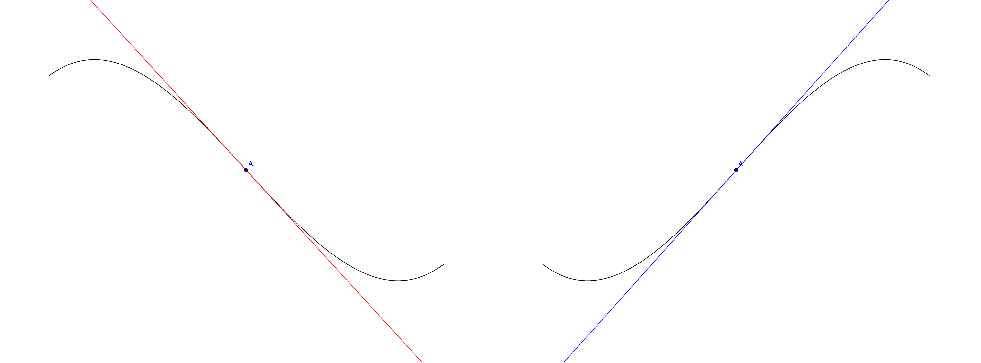
\includegraphics[height=3cm,bb=0 0 736 272,keepaspectratio=true]{./calculo/puntos_inflexion.png}
        % puntos_inflexion.png: 981x363 pixel, 96dpi, 25.95x9.60 cm, bb=0 0 736 272
        \caption{Puntos de inflexión}
        \label{fig:inflexion}
    \end{figure}


    \begin{figure}
        \centering
        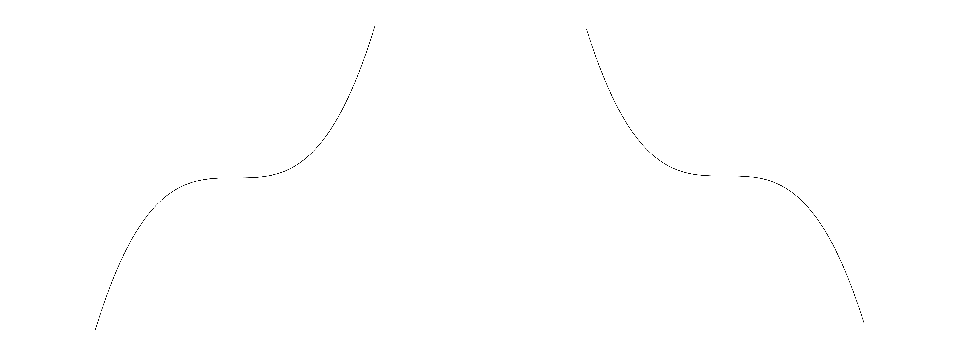
\includegraphics[height=3cm,bb=0 0 735 268,keepaspectratio=true]{./calculo/puntos_silla.png}
        % puntos_silla.png: 980x358 pixel, 96dpi, 25.93x9.47 cm, bb=0 0 735 268
        \caption{Puntos de silla}
        \label{fig:silla}
    \end{figure}



    Los puntos de inflexión pueden ser como en la figura \ref{fig:inflexion}. Si $f''$ cambia de negativa a positiva, la
    gráfica localmente como la de la izquierda, mientras que en el otro caso, luce como en la de la derecha.


    Falta por caracterizar los puntos críticos $c$ donde $f''(c)=0,$ es decir, que también son puntos de inflexión. Estos
    puntos se les conoce como \emph{puntos de silla} y alrededor de estos, la gráfica se ve como alguna de las de la figura
    \ref{fig:silla}.



    \begin{problema}
        \label{demo:grafica}
        Grafique la función $f:[-1,1]\to \R, f(x)=x^{3}-x.$
    \end{problema}


{Solución}
    
    Primero, resolvemos la ecuación
    $$
    x^3-x=0,
    $$
    y tenemos que las raíces de $f$ son $x=-1,0,1.$



    Después derivamos $f$:
    $$
    f'(x)=3x^{2}-1,
    $$
    y resolvemos la ecuación $f'(c)=0.$



    Entonces, los puntos críticos de la función son $x=\pm \frac{1}{\sqrt{3}}.$ Utilizamos el criterio
    \ref{criterio:segunda} para decidir si son máximo o mínimos locales, o incluso, puntos de silla.



    La segunda derivada de $f$ es
    $$
    f''(x)=6x.
    $$



    Como $f''(\frac{1}{\sqrt{3}})=6\left( \frac{1}{\sqrt{3}} \right)>0,$ entonces
    $$
    c=\dfrac{1}{\sqrt{3}}
    $$
    es un mínimo local.



    De manera similar, concluimos que
    $$
    c=-\dfrac{1}{\sqrt{3}}
    $$
    es un máximo local.



    Finalmente, resolvemos $f''(c)=0,$ pero la única solución es $c=0$ y por tanto, este es el único punto de inflexión.
    Como antes de $c=0,$ $f''<0,$ mientras que después $f''>,$ concluimos que en este punto, la gráfica se ve localmente
    como la gráfica de la derecha en la figura \ref{fig:inflexion}.



    \begin{figure}
        \centering
        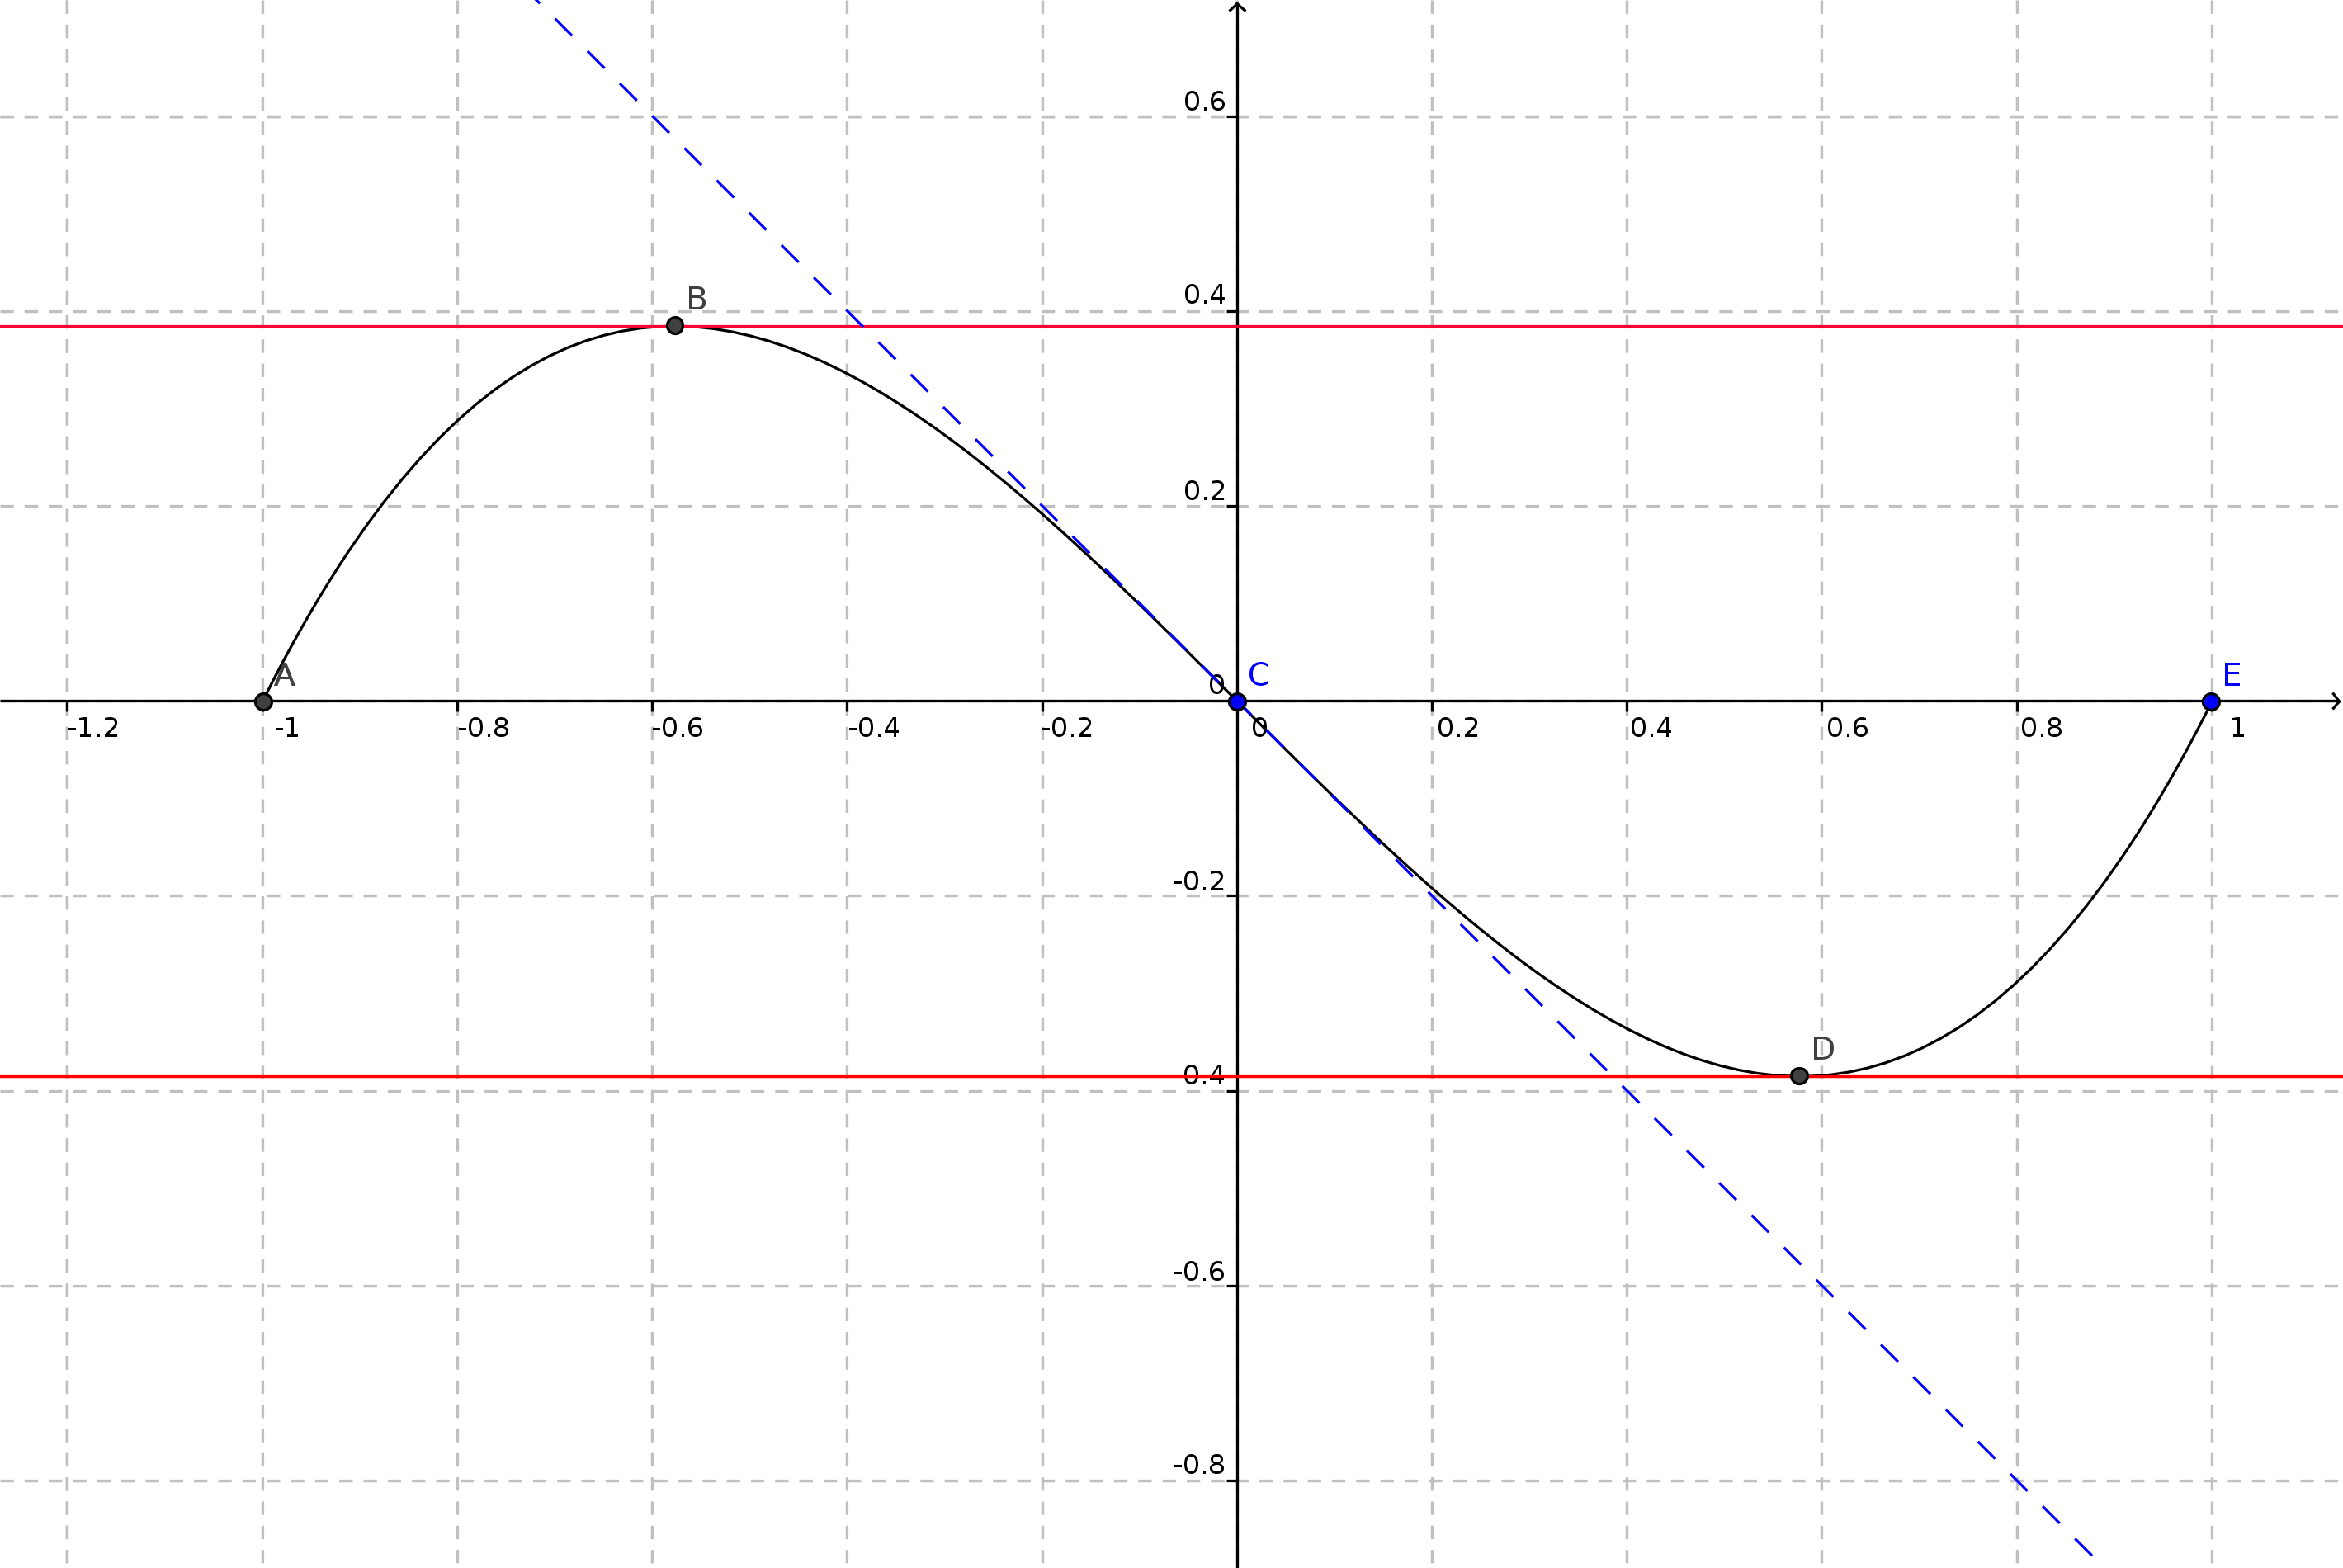
\includegraphics[height=5cm,bb=0 0 681 456,keepaspectratio=true]{./calculo/ejemplo_graficacion.png}
        % ejemplo_graficacion.png: 2839x1900 pixel, 300dpi, 24.04x16.09 cm, bb=0 0 681 456
        %\caption{Gráfica del ejericicio \ref{demo:grafica}}
        \label{fig:demo:grafica}
    \end{figure}


    
    Podemos utilizar \texttt{Sagemath} para graficar y comparar con nuestros resultados. La gráfica esta dada en la figura
    \ref{fig:demo:grafica}.
    

